\documentclass[a4paper,14pt, unknownkeysallowed]{extreport}

\usepackage{cmap} % Улучшенный поиск русских слов в полученном pdf-файле
\usepackage[T2A]{fontenc} % Поддержка русских букв
\usepackage[utf8]{inputenc} % Кодировка utf8
\usepackage[english,russian]{babel} % Языки: русский, английский
\usepackage{enumitem}


\usepackage{threeparttable}

\usepackage[14pt]{extsizes}

\usepackage{caption}
\captionsetup{labelsep=endash}
\captionsetup[figure]{name={Рисунок}}

% \usepackage{ctable}
% \captionsetup[table]{justification=raggedleft,singlelinecheck=off}

\usepackage{amsmath}

\usepackage{geometry}
\geometry{left=30mm}
\geometry{right=10mm}
\geometry{top=20mm}
\geometry{bottom=20mm}

\usepackage{titlesec}
\titleformat{\section}
	{\normalsize\bfseries}
	{\thesection}
	{1em}{}
\titlespacing*{\chapter}{0pt}{-30pt}{8pt}
\titlespacing*{\section}{\parindent}{*4}{*4}
\titlespacing*{\subsection}{\parindent}{*4}{*4}

\usepackage{setspace}
\onehalfspacing % Полуторный интервал

\frenchspacing
\usepackage{indentfirst} % Красная строка

\usepackage{titlesec}
\titleformat{\chapter}{\LARGE\bfseries}{\thechapter}{20pt}{\LARGE\bfseries}
\titleformat{\section}{\Large\bfseries}{\thesection}{20pt}{\Large\bfseries}

\usepackage{multirow}
\usepackage{listings}
\usepackage{xcolor}

% Для листинга кода:
\lstset{%
	language=Lisp,   					% выбор языка для подсветки	
	basicstyle=\small\sffamily,			% размер и начертание шрифта для подсветки кода
	numbers=left,						% где поставить нумерацию строк (слева\справа)
	numberstyle=\tiny,		     		% размер шрифта для номеров строк
	stepnumber=1,						% размер шага между двумя номерами строк
	numbersep=5pt,						% как далеко отстоят номера строк от подсвечиваемого кода
	frame=single,						% рисовать рамку вокруг кода
	tabsize=4,							% размер табуляции по умолчанию равен 4 пробелам
	captionpos=t,						% позиция заголовка вверху [t] или внизу [b]
	breaklines=true,					
	breakatwhitespace=true,				% переносить строки только если есть пробел
	backgroundcolor=\color{white},
	basicstyle=\footnotesize\ttfamily,
	keywordstyle=\color{blue},
	stringstyle=\color{red},
	commentstyle=\color{gray},
	showspaces=false,
    showstringspaces=false
}


\usepackage{pgfplots}
\usetikzlibrary{datavisualization}
\usetikzlibrary{datavisualization.formats.functions}


\lstset{
	literate=
	{а}{{\selectfont\char224}}1
	{б}{{\selectfont\char225}}1
	{в}{{\selectfont\char226}}1
	{г}{{\selectfont\char227}}1
	{д}{{\selectfont\char228}}1
	{е}{{\selectfont\char229}}1
	{ж}{{\selectfont\char230}}1
	{з}{{\selectfont\char231}}1
	{и}{{\selectfont\char232}}1
	{й}{{\selectfont\char233}}1
	{к}{{\selectfont\char234}}1
	{л}{{\selectfont\char235}}1
	{м}{{\selectfont\char236}}1
	{н}{{\selectfont\char237}}1
	{о}{{\selectfont\char238}}1
	{п}{{\selectfont\char239}}1
	{р}{{\selectfont\char240}}1
	{с}{{\selectfont\char241}}1
	{т}{{\selectfont\char242}}1
	{у}{{\selectfont\char243}}1
	{ф}{{\selectfont\char244}}1
	{х}{{\selectfont\char245}}1
	{ц}{{\selectfont\char246}}1
	{ч}{{\selectfont\char247}}1
	{ш}{{\selectfont\char248}}1
	{щ}{{\selectfont\char249}}1
	{ъ}{{\selectfont\char250}}1
	{ы}{{\selectfont\char251}}1
	{ь}{{\selectfont\char252}}1
	{э}{{\selectfont\char253}}1
	{ю}{{\selectfont\char254}}1
	{я}{{\selectfont\char255}}1
	{А}{{\selectfont\char192}}1
	{Б}{{\selectfont\char193}}1
	{В}{{\selectfont\char194}}1
	{Г}{{\selectfont\char195}}1
	{Д}{{\selectfont\char196}}1
	{Е}{{\selectfont\char197}}1
	{Ж}{{\selectfont\char198}}1
	{З}{{\selectfont\char199}}1
	{И}{{\selectfont\char200}}1
	{Й}{{\selectfont\char201}}1
	{К}{{\selectfont\char202}}1
	{Л}{{\selectfont\char203}}1
	{М}{{\selectfont\char204}}1
	{Н}{{\selectfont\char205}}1
	{О}{{\selectfont\char206}}1
	{П}{{\selectfont\char207}}1
	{Р}{{\selectfont\char208}}1
	{С}{{\selectfont\char209}}1
	{Т}{{\selectfont\char210}}1
	{У}{{\selectfont\char211}}1
	{Ф}{{\selectfont\char212}}1
	{Х}{{\selectfont\char213}}1
	{Ц}{{\selectfont\char214}}1
	{Ч}{{\selectfont\char215}}1
	{Ш}{{\selectfont\char216}}1
	{Щ}{{\selectfont\char217}}1
	{Ъ}{{\selectfont\char218}}1
	{Ы}{{\selectfont\char219}}1
	{Ь}{{\selectfont\char220}}1
	{Э}{{\selectfont\char221}}1
	{Ю}{{\selectfont\char222}}1
	{Я}{{\selectfont\char223}}1
}

\usepackage{graphicx}
\newcommand{\img}[3] {
	\begin{figure}[h!]
		\center{\includegraphics[height=#1]{img/#2}}
		\caption{#3}
		\label{img:#2}
	\end{figure}
}


\usepackage[justification=centering]{caption} % Настройка подписей float объектов

\usepackage[unicode,pdftex]{hyperref} % Ссылки в pdf
\hypersetup{hidelinks}

\usepackage{csvsimple}

\newcommand{\code}[1]{\texttt{#1}}

\usepackage{longtable}

\usepackage{array}
\usepackage{booktabs}
\usepackage{floatrow}

\floatsetup[longtable]{LTcapwidth=table}

% \def\UrlBreaks{\do\/\do-\do\_}

\makeatletter
\renewcommand*\l@chapter[2]{%
  \ifnum \c@tocdepth >\m@ne
    \addpenalty{-\@highpenalty}%
    \vskip 1.0em \@plus\p@
    \setlength\@tempdima{1.5em}%
    \begingroup
      \parindent \z@ \rightskip \@pnumwidth
      \parfillskip -\@pnumwidth
      \leavevmode \bfseries
      \advance\leftskip\@tempdima
      \hskip -\leftskip
      #1\nobreak\normalfont\leaders\hbox{$\m@th
        \mkern \@dotsep mu\hbox{.}\mkern \@dotsep
        mu$}\hfill\nobreak\hb@xt@\@pnumwidth{\hss #2}\par
      \penalty\@highpenalty
    \endgroup
  \fi}
\makeatother

\begin{document}



\begin{titlepage}
	\newgeometry{pdftex, left=2cm, right=2cm, top=2.5cm, bottom=2.5cm}
	\fontsize{12pt}{12pt}\selectfont
	\noindent \begin{minipage}{0.15\textwidth}
		
\includegraphics[width=\linewidth]{img/b_logo.jpg}
	\end{minipage}
	\noindent\begin{minipage}{0.9\textwidth}\centering
		\textbf{Министерство науки и высшего образования Российской Федерации}\\
		\textbf{Федеральное государственное бюджетное образовательное учреждение высшего образования}\\
		\textbf{«Московский государственный технический университет имени Н. Э.~Баумана}\\
		\textbf{(национальный исследовательский университет)»}\\
		\textbf{(МГТУ им. Н. Э.~Баумана)}
	\end{minipage}
	
	\noindent\rule{18cm}{3pt}
	\newline\newline
	\noindent ФАКУЛЬТЕТ $\underline{\text{«Информатика и системы управления»~~~~~~~~~~~~~~~~~~~~~~~~~~~~~~~~~~~~~~~~~~~~~~~~~~~~~~~}}$ \newline\newline
	\noindent КАФЕДРА $\underline{\text{«Программное обеспечение ЭВМ и информационные технологии»~~~~~~~~~~~~~~~~~~~~~~~}}$\newline\newline\newline\newline\newline\newline\newline
	
	
	\begin{center}
		\noindent\begin{minipage}{1.3\textwidth}\centering
		\Large\textbf{   ~~~ Лабораторная работа №2}\newline
		\textbf{по курсу "Функциональное}\newline
		\textbf{и логическое программирование"}\newline\newline\newline
		\end{minipage}
	\end{center}
	
	\noindent\textbf{Тема} 			$\underline{\text{Определение функций пользователя}}$\newline\newline
	\noindent\textbf{Студент} 		$\underline{\text{Ковалец К. Э.}}$\newline\newline
	\noindent\textbf{Группа} 		$\underline{\text{ИУ7-63Б}}$\newline\newline
	\noindent\textbf{Преподаватели} $\underline{\text{Толпинская Н. Б., Строганов Ю. В.}}$\newline
	
	\begin{center}
		\vfill
		Москва~---~\the\year
		~г.
	\end{center}
	\restoregeometry
\end{titlepage}



\setcounter{page}{2}
\chapter{Практические задания}

Все диаграммы вычислений приложены к отчету.

\section{Задание 1}

Составить диаграмму вычисления следующих выражений.

\begin{center}
\captionsetup{justification=raggedright,singlelinecheck=off}
\begin{lstlisting}[label=lst:parallel_processing,caption=Выражения для построения диаграмм в задании 1]
(equal 3 (abs - 3)) 
(equal (+ 1 2) 3) 
(equal (* 4 7) 21)
(equal (* 2 3) (+ 7 2)) 
(equal (- 7 3) (* 3 2)) 
(equal (abs (- 2 4)) 3))
\end{lstlisting}
\end{center}

\section{Задание 2}

Написать функцию, вычисляющую гипотенузу прямоугольного треугольника по заданным катетам и составить диаграмму её вычисления.

\begin{center}
\captionsetup{justification=raggedright,singlelinecheck=off}
\begin{lstlisting}[label=lst:parallel_processing,caption=Решение задания 2]
(defun hypotenuse(a b) (sqrt (+ (* a a) (* b b))))
;; (HYPOTENUSE 3 4) -> 5.0
\end{lstlisting}
\end{center}

\section{Задание 3}

Написать функцию, вычисляющую объем параллелепипеда по 3-м его сторонам, и составить диаграмму ее вычисления.

\begin{center}
\captionsetup{justification=raggedright,singlelinecheck=off}
\begin{lstlisting}[label=lst:parallel_processing,caption=Решение задания 3]
(defun volume(a b c) (* a b c))
;; (VOLUME 2 3 4) -> 24
\end{lstlisting}
\end{center}

\section{Задание 4}

Каковы результаты вычисления следующих выражений? (объяснить возможную ошибку и варианты ее устранения)

\begin{center}
\captionsetup{justification=raggedright,singlelinecheck=off}
\begin{lstlisting}[label=lst:parallel_processing,caption=Решение задания 4]
(list 'a c)         ;; The variable C is unbound.
(cons 'a (b c))     ;; The variable C is unbound
(cons 'a '(b c))    ;; (A B C)
(caddy (1 2 3 4 5)) ;; Execution of a form compiled with errors.
(cons 'a 'b 'c)     ;; invalid number of arguments: 3
(list 'a (b c))     ;; The variable C is unbound.
(list a '(b c))     ;; The variable A is unbound.
(list (+ 1 '(length '(1 2 3)))) ;; The value (LENGTH '(1 2 3)) is not of type NUMBER
\end{lstlisting}
\end{center}

\begin{center}
\captionsetup{justification=raggedright,singlelinecheck=off}
\begin{lstlisting}[label=lst:parallel_processing,caption=Варианты следующих выражений с устраненными ошибками]
(list 'a 'c)         ;; (A C)
(cons 'a '(b c))     ;; (A B C)
(cons 'a '(b c))     ;; (A B C)
(caddr '(1 2 3 4 5)) ;; 3
(cons 'a 'b)         ;; (A . B)
(list 'a '(b c))     ;; (A (B C))
(list 'a '(b c))     ;; (A (B C))
(list (+ 1 (length '(1 2 3)))) ;; (4)
\end{lstlisting}
\end{center}

\section{Задание 5}

Написать функцию $longer\_then$ от двух списков-аргументов, которая возвращает $T$, если первый аргумент имеет большую длину.

\begin{center}
\captionsetup{justification=raggedright,singlelinecheck=off}
\begin{lstlisting}[label=lst:parallel_processing,caption=Решение задания 5]
(defun longer_then(list1 list2) 
	(> (length list1) (length list2)))
;; (LONGER_THEN '(1 2 3) '(1 2)) -> T
;; (LONGER_THEN '(1 2 3) '(1 2 3)) -> NIL
;; (LONGER_THEN '(1 2 3) '(1 2 3 4)) -> NIL
\end{lstlisting}
\end{center}

\section{Задание 6}

Каковы результаты вычисления следующих выражений?\newline

В 4-ом выражении была исправлена ошибка. Изначально было так:
\begin{center}
\captionsetup{justification=raggedright,singlelinecheck=off}
\begin{lstlisting}[label=lst:parallel_processing,caption=Исходное 4-ое выражение]
(+ (length for 2 too)) (car '(21 22 23))) ;;  The variable FOR is unbound.
\end{lstlisting}
\end{center}

\begin{center}
\captionsetup{justification=raggedright,singlelinecheck=off}
\begin{lstlisting}[label=lst:parallel_processing,caption=Решение задания 6]
(cons 3 (list 5 6))             ;; (3 5 6)
(cons 3 '(list 5 6))            ;; (3 LIST 5 6)
(list 3 'from 9 'lives (- 9 3)) ;; (3 FROM 9 LIVES 6)
(+ (length '(for 2 too)) (car '(21 22 23))) ;; 24
(cdr '(cons is short for ans))  ;; (IS SHORT FOR ANS)
(car (list one two))            ;; The variable ONE is unbound.
(car (list 'one 'two))          ;; ONE
\end{lstlisting}
\end{center}

\section{Задание 7}

Дана функция \texttt{(defun mystery (x) (list (second x) (first x)))}. Какие результаты вычисления следующих выражений?

\begin{center}
\captionsetup{justification=raggedright,singlelinecheck=off}
\begin{lstlisting}[label=lst:parallel_processing,caption=Решение задания 7]
(mystery (one two))      ;; The variable TWO is unbound. 
(mystery one 'two))      ;; The variable ONE is unbound.
(mystery (last one two)) ;; The variable ONE is unbound.
(mystery free)           ;; The variable FREE is unbound.	
\end{lstlisting}
\end{center}

\begin{center}
\captionsetup{justification=raggedright,singlelinecheck=off}
\begin{lstlisting}[label=lst:parallel_processing,caption=Варианты следующих выражений с устраненными ошибками]
(mystery '(one two))        ;; (TWO ONE) 
(mystery '(one 'two))       ;; ('TWO ONE) 
(mystery (last '(one two))) ;; (NIL TWO)
(mystery '(free))           ;; (NIL FREE)
\end{lstlisting}
\end{center}

\section{Задание 8}

Написать функцию, которая переводит температуру в системе Фаренгейта температуру по Цельсию \texttt{(defun f-to-c (temp)...)}.

Формулы: $c = 5/9*(f-32.0); \ f= 9/5*c+32.0$.

Как бы назывался роман Р. Брэдбери "+451 по Фаренгейту" \ в системе по Цельсию?

\begin{center}
\captionsetup{justification=raggedright,singlelinecheck=off}
\begin{lstlisting}[label=lst:parallel_processing,caption=Решение задания 8]
(defun f-to-c (temp) (* (/ 5 9) (- temp 32.0)))
;; (F-TO-C 451) -> 232.77779
\end{lstlisting}
\end{center}

Роман Р. Брэдбери назывался бы "+232.77779 по Цельсию".

\section{Задание 9}

Что получится при вычисления каждого из выражений?\newline

В 4-ом выражении была исправлена ошибка. Изначально было так:
\begin{center}
\captionsetup{justification=raggedright,singlelinecheck=off}
\begin{lstlisting}[label=lst:parallel_processing,caption=Исходное 4-ое выражение]
(apply #cons "(t NIL)) ;; illegal complex number format: #CONS
\end{lstlisting}
\end{center}


\begin{center}
\captionsetup{justification=raggedright,singlelinecheck=off}
\begin{lstlisting}[label=lst:parallel_processing,caption=Решение задания 9]
(list 'cons t NIL)               ;; (CONS T NIL)
(eval (list 'cons t NIL))        ;; (T)
(eval (eval (list 'cons t NIL))) ;; The function T is undefined, and its name is reserved by ANSI CL.
(apply #'cons '(t NIL))          ;; (T)
(eval NIL)                       ;; NIL
(list 'eval NIL)                 ;; (EVAL NIL)
(eval (list 'eval NIL))          ;; NIL
\end{lstlisting}
\end{center}

\section{Дополнительные задания}

\subsection{Написать функцию, вычисляющую катет по заданной гипотенузе и другому катету прямоугольного треугольника, и составить диаграмму ее вычисления.}

\begin{center}
\captionsetup{justification=raggedright,singlelinecheck=off}
\begin{lstlisting}[label=lst:parallel_processing,caption=Решение дополнительного задания 1]
(defun calc_cathet (hypotenuse cathet)
	(sqrt (- (* hypotenuse hypotenuse) (* cathet cathet))))
;; (CALC_CATHET 5 4) -> 3.0
\end{lstlisting}
\end{center}

\subsection{Написать функцию, вычисляющую площадь трапеции по ее основаниям и высоте, и составить диаграмму ее вычисления.}

\begin{center}
\captionsetup{justification=raggedright,singlelinecheck=off}
\begin{lstlisting}[label=lst:parallel_processing,caption=Решение дополнительного задания 2]
(defun trapezoid_area (h a b) 
	(* (/ (+ a b) 2) h))
;; (TRAPEZOID_AREA 2 3 4) -> 7
\end{lstlisting}
\end{center}


\chapter{Ответы на теоретические вопросы к лабораторной работе}

\section{Базис Lisp}

\textbf{Базис языка} -- минимальный набор конструкций языка и структур данных, с помощью которых можно решить любую задачу.

Базис языка Lisp содержит:

\begin{itemize}
	\item атомы и структуры (представляющиеся бинарными узлами);
	\item базовые функции и функционалы:
	\begin{itemize}
		\item встроенные -- примитивные функции (atom, eq, cons, car, cdr);
		\item специальные функции и функционалы (quote, cond, lambda, eval, apply, funcall).
	\end{itemize}
\end{itemize}

\section{Классификация функций}

Функции в Lisp классифицируют следующим образом:

\begin{itemize}
	\item чистые математические функции;
	\item рекурсивные функции;
	\item специальные функции -- формы (прнимают произвольное число аргументов или по разному обрабатывают аргументы);
	\item псевдофункции (создают эффект на внешнем устройстве);
	\item функции с вариативными значениями, из которых выбирается одно;
	\item функции высших порядков -- функционалы (используются для построения синтаксически управляемых программ).
\end{itemize}

По назначению функции разделяются следующим образом:

\begin{itemize}
	\item конструкторы — создают значение (cons, list);
	\item селекторы — получают доступ по адресу (car, cdr); 
	\item предикаты — возвращают Nil, T.
\end{itemize}

\section{Способы создания функций}

\textbf{Функцией} называется правило, по которому каждому значению одного или нескольких аргументов ставится в соответствие конкретное значение результата.

\begin{itemize}
	\item В Lisp можно определить функцию без имени с помощью \textbf{$\lambda$-выражений}. 
	Lambda-определение безымянной функции:
	
	\begin{center}
	\texttt{(lambda <lambda-список> <форма>)}
	\end{center}

	Lambda-вызов функции:

	\begin{center}
	\texttt{(<lambda-выражение> <формальные параметры>)}
	\end{center}

	\item Также в Lisp можно определить функцию с именем с помощью \textbf{defun}. В таких функциях defun связывает символьный атом с Lambda-определением:
	
	\begin{center}
	\texttt{(defun f <lambda-выражение>)}
	\end{center}

	Упрощенное определение:

	\begin{center}
	\texttt{(defun f(arg1, ..., argN) <формы>)}
	\end{center}

\end{itemize}

\section{Функции Car и Cdr}

Функции \textbf{car}, \textbf{cdr} являются базовыми функциями доступа к данным. 

\begin{itemize}
	\item \textbf{car} принимает точечную пару или список в качестве аргумента и возвращает первый элемент или Nil, соответственно. 
	\item \textbf{cdr} принимает точечную пару или список в качестве аргумента и возвращает все элементы кроме первого или Nil, соответственно.
\end{itemize}

\section{Назначение и отличие в работе Cons и List}

Функции \textbf{list}, \textbf{cons} являются функциями создания списков (cons – базовая, list – нет). 

\begin{itemize}
	\item \textbf{cons} создает списочную ячейку и устанавливает два указателя на аргументы.
	
	\begin{figure}[h]
		\centering
		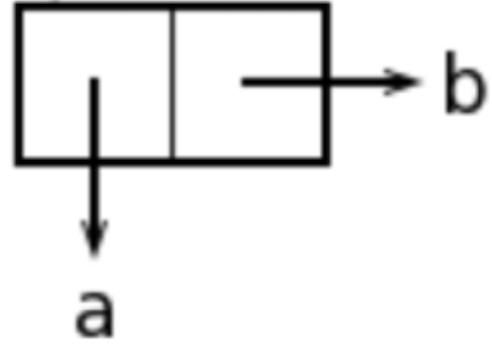
\includegraphics[scale=0.4]{img/picture1.png}
		\caption{Результат $cons$}
		\label{fig:picture1}
	\end{figure} 
	
	\item \textbf{list} принимает переменное число аргументов и возвращает список, элементы которого -- переданные в функцию аргументы.
	
	\begin{figure}[h]
		\centering
		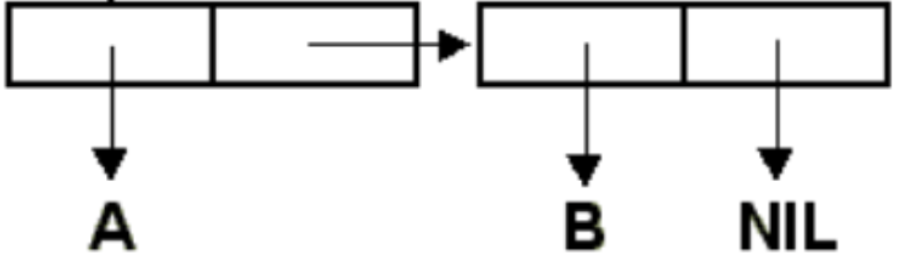
\includegraphics[scale=0.45]{img/picture2.png}
		\caption{Результат $list$}
		\label{fig:picture2}
	\end{figure} 

\end{itemize} 

\end{document}
